\documentclass[tikz,border=6pt]{standalone}

\usepackage{fontspec}
\usepackage{unicode-math}
\setmainfont{DejaVu Serif}
\setsansfont{DejaVu Sans}
\setmathfont{latinmodern-math.otf}

\usepackage{pgfplots}
\pgfplotsset{compat=1.18}
\usepackage{array}
\usetikzlibrary{calc}

\begin{document}

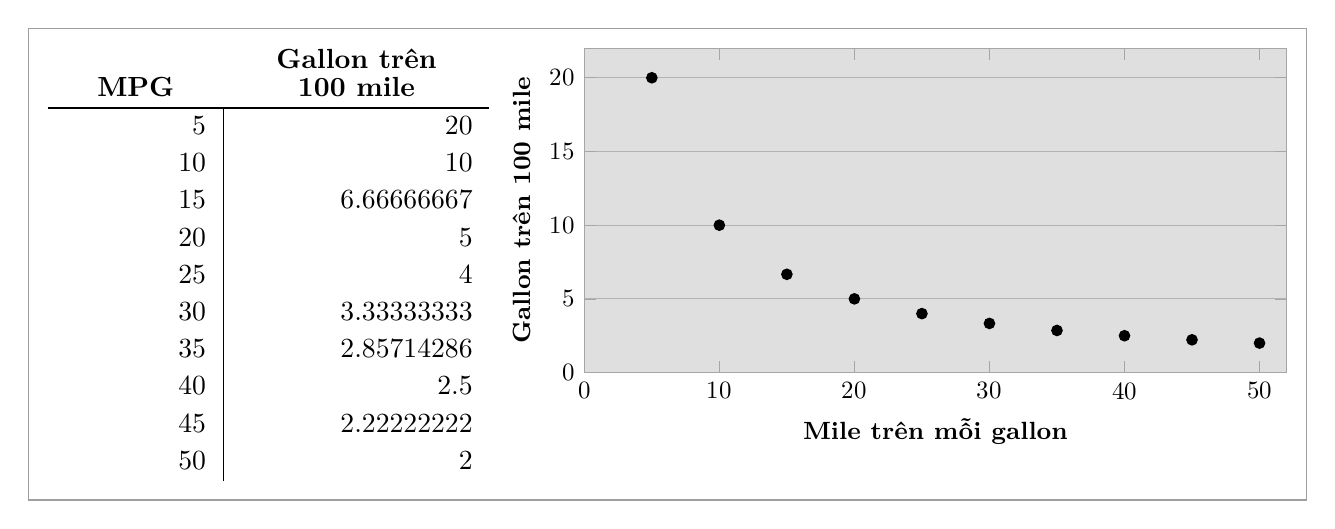
\begin{tikzpicture}

% -----------------------------
% Bảng số liệu
% -----------------------------
\node[anchor=north west, inner sep=0pt] (tbl) at (0,0) {%
  \renewcommand{\arraystretch}{1.12}%
  \begin{tabular}{>{\raggedleft\arraybackslash}p{1.8cm}|>{\raggedleft\arraybackslash}p{2.95cm}}
    \multicolumn{1}{c}{\textbf{\shortstack{MPG}}} & \multicolumn{1}{c}{\textbf{\shortstack{Gallon trên\\100 mile}}} \\
    \hline
    5  & 20 \\
    10 & 10 \\
    15 & 6.66666667 \\
    20 & 5 \\
    25 & 4 \\
    30 & 3.33333333 \\
    35 & 2.85714286 \\
    40 & 2.5 \\
    45 & 2.22222222 \\
    50 & 2 \\
  \end{tabular}%
};

% -----------------------------
% Biểu đồ phân tán
% -----------------------------
\begin{axis}[
  at={($(tbl.north east)+(1.2cm,0cm)$)},
  anchor=north west,
  width=10.5cm,
  height=5.7cm,
  xmin=0,
  xmax=52,
  ymin=0,
  ymax=22,
  xtick={0,10,20,30,40,50},
  ytick={0,5,10,15,20},
  xlabel={\textbf{Mile trên mỗi gallon}},
  ylabel={\textbf{Gallon trên 100 mile}},
  axis background/.style={fill=gray!25},
  axis line style={draw=gray!70},
  tick style={draw=gray!70},
  ymajorgrids=true,
  xmajorgrids=false,
  major grid style={draw=gray!60, line width=0.4pt},
  tick label style={font=\small},
  label style={font=\small},
  enlargelimits=false,
  clip=false
]
\addplot[
  only marks,
  mark=*,
  mark size=1.9pt,
  color=black
] coordinates {
  (5,20)
  (10,10)
  (15,6.66666667)
  (20,5)
  (25,4)
  (30,3.33333333)
  (35,2.85714286)
  (40,2.5)
  (45,2.22222222)
  (50,2)
};
\end{axis}

% -----------------------------
% Khung ngoài toàn hình
% -----------------------------
\draw[gray!75, line width=0.5pt]
  ([xshift=-7pt,yshift=7pt]current bounding box.north west)
  rectangle
  ([xshift=7pt,yshift=-7pt]current bounding box.south east);

\end{tikzpicture}

\end{document}
